\chapter{Cahier des besoins}

\section{Besoins fonctionnels}

\subsection{Besoin Utilisateurs}
\subsubsection{Créer des routes}
L'application doit permettre de créer des routes dans le réseau, c'est-à-dire de trouver un chemin allant du routeur d'entrée vers une autre cible. Il faudra donc modifier la table de routage du routeur d'entrée. Dans notre cas, la cible sera une adresse fictive et permettra un routage vers un trou noir pour contrer l'attaque.
\subparagraph{Protocole de test :}
\begin{itemize}
    \item Création d'une route.
    \item Création d'une route avec arguments invalide.
\end{itemize}
\subparagraph{Résultat obtenu :}
    \begin{itemize}
    \item Route créée.
    \item Aucune autre route n'a été créée.
    \item Aucune route n'a été détruite.
    \item Aucune modification sur l'état des autres routes.
    \item Message d'erreur si arguments invalide.
\end{itemize}
\subparagraph{Conclusion :}Ce besoin est correctement rempli.

\subsubsection{Supprimer des routes}
Puisqu'il permet la création, l'application devra permettre également la suppression des routes précédemment créées.
\subparagraph{Protocole de test :}
\begin{itemize}
    \item Suppression d'une route.
    \item Suppression d'une route avec arguments invalide.
\end{itemize}
\subparagraph{Résultat obtenu :}
    \begin{itemize}
    \item Route supprimée.
    \item Aucune route n'a été créée.
    \item Aucune autre route n'a été détruite.
    \item Aucune modification sur l'état des autres routes.
    \item Message d'erreur si arguments invalide.
\end{itemize}
\subparagraph{Conclusion :}Ce besoin est correctement rempli.

\subsubsection{Activer \& désactiver des routes}
Une fonction d'activation et de désactivation des routes existantes permettra de gérer les routes existantes sans les supprimer et donc sans avoir besoin de les recréer par la suite.
\subparagraph{Protocole de test :}
\begin{itemize}
    \item Activation d'une route.
    \item Désactivation d'une route.
    \item Action sur route invalide.
\end{itemize}
\subparagraph{Résultat obtenu :}
    \begin{itemize}
    \item État de la route modifiée.
    \item Aucune route n'a été créée.
    \item Aucune route n'a été détruite.
    \item Aucune modification sur l'état des autres routes.
    \item Message d'erreur et suppression de la base donnée si arguments invalide.
\end{itemize}
\subparagraph{Conclusion :}Ce besoin est correctement rempli.

\subsubsection{Importer \& exporter des routes}
Un système d'import et d'export doit être mis en place. Cela permettra à l'utilisateur de sauvegarder l'état des routes dans un fichier puis de les réimporter plus tard.

\subsubsection{Connexions \& Déconnexions}
Une page d'authentification permettra de restreindre l'accès de l'application et donc permettre que l'administrateur soit le seul à pouvoir se connecter.
\subparagraph{Protocole de test :}
\begin{itemize}
    \item Connexion de l'administrateur.
    \item Déconnexion de l'administrateur.
\end{itemize}
\subparagraph{Résultat obtenu :}
    \begin{itemize}
    \item État de la connexion modifié.
    \item L'administrateur a accès aux fonctionnalités après une connexion réussie.
    \item Retour à la page de connexions après une déconnexion réussie.
    \item Aucune autre modification.
\end{itemize}
\subparagraph{Conclusion :}Ce besoin est correctement rempli.

\subsection{Interface utilisateur}
\label{sssec:ui}

Pour permettre une gestion plus simplifiée des différentes fonctions demandées tout en gardant un visuel sur la situation actuelle, une interface graphique est nécessaire.

L'interface graphique que l'utilisateur va utiliser est une application Web, un client léger, qui est dépendante d'un serveur pour fonctionner correctement.\newline

\begin{figure}[H]
    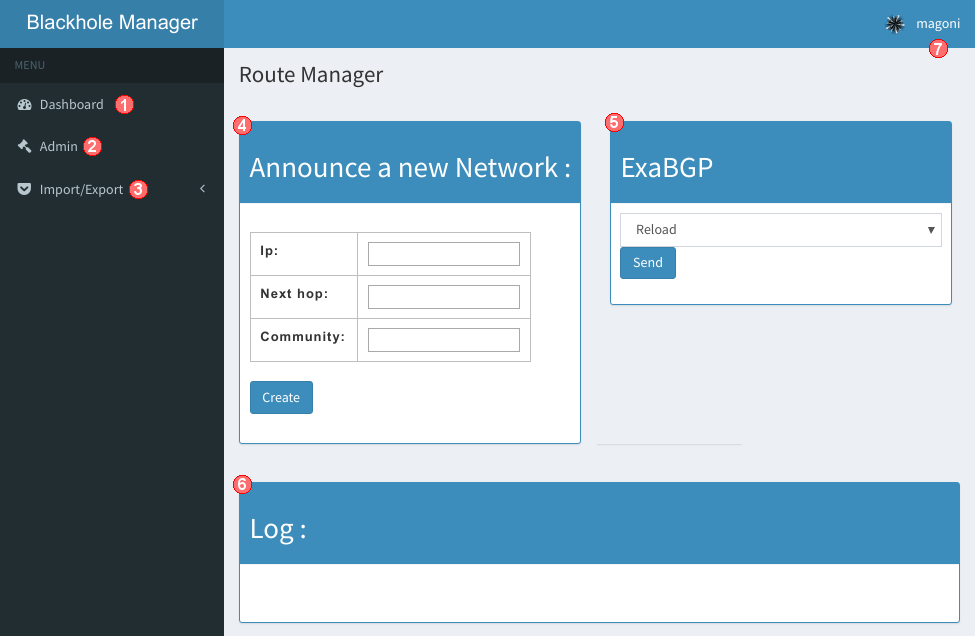
\includegraphics[width=\textwidth]{medias/ui_upper_marked.png}
    \caption{Interface utilisateur}
    \label{fig:ui_upper}
\end{figure}

\newpage
\textbf{Lien "Dashboard"} (1)\newline
Ce lien permet d'être redirigé vers cette page. Il peut être utile si l'utilisateur veut recharger la page ou s'il se trouve sur la page de changement de mot de passe.\newline

\textbf{Lien "Admin"} (2)\newline
Ce lien permet d'accéder à la page d'administration de l'application.\newline

\textbf{Déroulant "Import/Export"} (3)\newline
Ce déroulant permet d'afficher les boutons "Import" et "Export". 
\begin{itemize}
    \item Le bouton "Import" permet d'importer des routes contenue dans un fichier. Lorsque l'on utilise ce bouton, un gestionnaire de fichier se lance et il faut sélectionner un fichier contenants des routes au format JSON.
    \item Le bouton "Export" permet d'exporter toutes les routes de la page dans un fichier. Lorsque l'on utilise ce bouton, une zone de texte apparaît et il suffit d'écrire le chemin ou exporter les routes. L'export se fait dans un fichier "data.json" et les routes sont écrite en format JSON.\newline
\end{itemize}

\textbf{Boite "Announce a new Network"} (4)\newline
Cette boite permet de créer et d'envoyer à l'api la nouvelle route que l'on souhaite créer. Il suffit de remplir les champs en suivants les règles syntaxiques liés à chaque champ.
\begin{itemize}
    \item "Ip" doit être du format "192.168.0.1/32".
    \item "Next hop" doit être du format "192.168.0.1".
    \item "Community" doit être du format "45:50" mais peut aussi être vide.\newline
\end{itemize}

\textbf{Boite "ExaBGP"} (5)\newline
Cette boite permet d'envoyer à l'api les commandes ExaBGP que l'on veut qu'elle lance. Il suffit de choisir la commande dans la liste déroulante puis de appuyer sur "Send". Si une réponse de l'api est attendue, elle s'affichera dans la boite "Log".\newline

\textbf{Boite "Log"} (6)\newline
Cette boite contient les dernières informations sur les actions effectuée. Elle permet à l'utilisateur de savoir si l'action s'est bien passé ou d'obtenir le code d'erreur le cas échéant.
Elle permet aussi d'obtenir le résultat des commandes ExaBGP.\newline

\textbf{Menu utilisateur} (7)\newline
Ce bouton permet de faire apparaître un petit menu pour permettre à l'utilisateur de se déconnecter ou de changer son mot de passe.

\begin{figure}[H]
    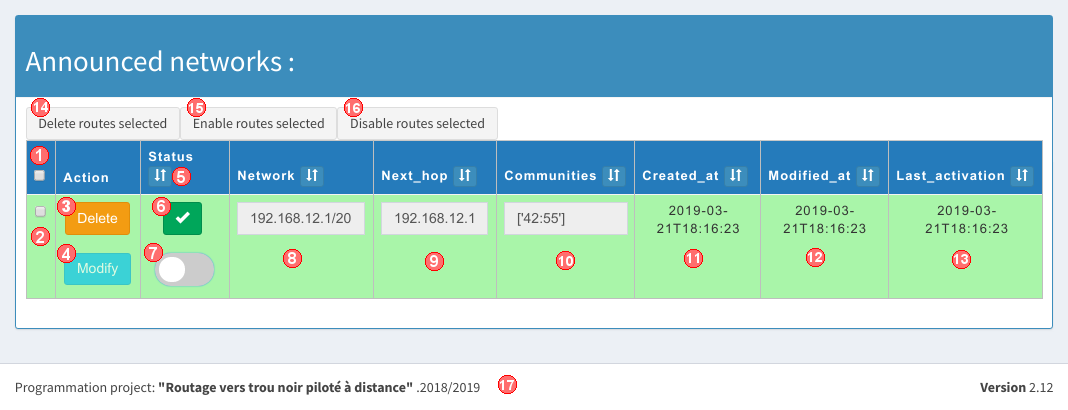
\includegraphics[width=\textwidth]{medias/ui_lower_marked.png}
    \caption{Interface utilisateur}
    \label{fig:ui_lower}
\end{figure}

%Image route
\textbf{Case à cocher globale} (1)\newline
Cette case à cocher permet de sélectionner (ou désélectionner) l'intégralitée des routes présente sur la page.\newline

\textbf{Case à cocher} (2)\newline
Cette case à cocher est associée à une seule route et permet donc de sélectionner (ou désélectionner) la route pour lui appliquer un traitement en parallèle d'autres routes.\newline

\textbf{Bouton "Delete"} (3)\newline
Ce bouton est associée à une seule route et permet donc de supprimer la route associée.\newline

\textbf{Bouton "Modify"} (4)\newline
Ce bouton est associée à une seule route et permet donc de modifier la route associée. Les modifications appliquées seront celles explicitées dans les zones de textes associées. Ce bouton est désactivé le temps que le "Unlock" de la route ne seras pas activé. \newline

\textbf{Bouton de tri} (5)\newline
Ce bouton, existant pour chaque colonne, permet de faire un tri sur la colonne associée. Un premier "click" permettra de faire le tri et un second et d'inverser l'autre du tri. Ce tri reviendra à zéro ou sera remplacé par un autre tri si une autre action venant à recharger la page ou un tri sur une autre colonne est mis en oeuvre.\newline

\textbf{Bouton Activer/Désactiver} (6)\newline
Ce bouton est associée à une seule route et permet donc de d'activer ou désactiver la route associée. Selon l'état de la route, le bouton changera:
\begin{itemize}
    \item Si la route est activée, le bouton sera vert (Tout comme le fond de la route) et un "click" permettra de désactiver la route.
    \item Si la route est désactivée, le bouton sera rouge (Tout comme le fond de la route) et un "click" permettra d'activer la route.\newline
\end{itemize}

\textbf{Bouton "Unlock"} (7)\newline
Ce bouton est associée à une seule route et permet donc d'activer ou désactiver la sécurité pour la modification. Cette sécurité évite de modifier une route pas inadvertance. Une fois activée, l'utilisateur peut modifier la route associée et l'envoyer en utilisant le bouton "Modify".\newline

\textbf{Zone de texte "Network"} (8)\newline
Cette zone de texte contient de base la valeur courante de "Network" dans la base donnée pour la route associée. Une fois le "Unlock" activé, il est possible de modifier ce champs pour modifier la route associée.\newline

\textbf{Zone de texte "Next\_hop"} (9)\newline
Cette zone de texte contient de base la valeur courante de "Next\_hop" dans la base donnée pour la route associée. Une fois le "Unlock" activé, il est possible de modifier ce champs pour modifier la route associée.\newline

\textbf{Zone de texte "Communities"} (10)\newline
Cette zone de texte contient de base la valeur courante de "Communities" dans la base donnée pour la route associée. Une fois le "Unlock" activé, il est possible de modifier ce champs pour modifier la route associée.\newline

\textbf{Texte "Created\_at"} (11)\newline
Ce texte contient de base la valeur courante de "Created\_at" dans la base donnée pour la route associée.\newline

\textbf{Texte "Modified\_at"} (12)\newline
Ce texte contient de base la valeur courante de "Modified\_at" dans la base donnée pour la route associée.\newline

\textbf{Texte "Last\_activation"} (13)\newline
Ce texte contient de base la valeur courante de "Last\_activation" dans la base donnée pour la route associée.\newline

\textbf{Bouton "Delete routes selected"} (14)\newline
Ce bouton permet de supprimer toutes les routes qui sont sélectionnées par leurs "case à cocher" cochées.\newline

\textbf{Bouton "Enable routes selected"} (15)\newline
Ce bouton permet d'activer toutes les routes qui sont sélectionnées par leurs "case à cocher" cochées.\newline

\textbf{Bouton "Disable routes selected"} (16)\newline
Ce bouton permet de désactiver toutes les routes qui sont sélectionnées par leurs "case à cocher" cochées.\newline

\textbf{Pied de page} (17)\newline
Le pied de page permet de signaler à l'utilisateur la version actuelle de l'application.

%\textbf{Voyant coloré} (1)\newline
%Il faut indiquer à l'utilisateur si le client est actuellement connecté à l'API, ce qui sera représenté par un voyant coloré en haut de la page. Le "\textit{Vert}" signifie que le client est connecté. Le "\textit{Rouge}" signifie que le client est déconnecté et que toutes les modifications effectuées pendant cette période de déconnexion seront perdues.
%Le client vérifie périodiquement (chaque seconde) qu'il est toujours connecté à l'API en faisant une requête (rapide).
%S'il reçoit une réponse, le voyant coloré deviens vert.
%Dans le cas où il ne recevrait pas de réponse, le voyant coloré deviens rouge jusqu'au rétablissement de la connexion.\newline

%\textbf{Déconnexion} (2)\newline
%Permet à un utilisateur authentifié de se déconnecter.
%Dans le cas où il existerait plusieurs compte utilisateur, il serait possible d'afficher l'identité de l'utilisateur actuel à cet emplacement.\newline

%\textbf{Annoncer un nouveau réseau ou une IP} (3)\newline
%Un formulaire permettra à l'utilisateur de créer des routes. Ces routes serviront à rediriger des attaques dans un trou noir selon leur origine et des communautés de routeurs. Le formulaire est composé de trois éléments.

% \textit{L'adresse IP ou Réseau de l'attaquant} (4), un champ textuel où l'utilisateur pourra écrire.
% Si la source de l'attaque est une adresse IP, l'utilisateur devra écrire son adresse IP en notation IPv4.
% Si la source de l'attaque est un réseau, l'utilisateur devra respecter la notation IPv4 et CIDR, sinon la validation sera impossible. Il serait pertinent de relier cet élément à l'application du groupe "détection des attaques DDoS" afin d'éviter à l'utilisateur d'aller chercher ces informations.
% Un champ textuel avec de l'autocomplétion pourrait être adapté.

% \textit{L'adresse du prochain saut vers un trou noir} (5), une liste déroulante où l'utilisateur pourra sélectionner un élément parmi plusieurs. Dans le cas où les "prochain saut" sont toujours des interfaces null, cet élément peut être facultatif.

% \textit{La communauté de routeurs qui va utiliser cette route} (6), une liste avec des éléments à cocher où l'utilisateur pourra sélectionner quelques élément parmi plusieurs.
% Quand un élément de la liste est sélectionné, sa couleur passe du blanc (7) au vert (8).

% Quand l'utilisateur a fini de remplir le formulaire, il pourra cliquer sur le bouton valider (9).
% Ce qui fera apparaître une fenêtre de confirmation contenant un résumé du formulaire de création de route.
% Une fenêtre de confirmation permet de limiter les erreurs de manipulations, en demandant à l'utilisateur de cliquer à deux endroits différents.\newline

% \textbf{Sous-réseaux annoncés} (10)\newline
% Une liste permettra à l'utilisateur de consulter les routes existantes.

% %1 : synchronisation du contenu
% Cette liste sera mise à jour au lancement de l'application, lors de chaque modification et à la demande de l'utilisateur à l'aide d'un bouton (11) pour rafraîchir le contenu de la liste.
% La synchronisation de la liste pourrait être effectuée de deux manières.

% % tout récupérer = gros lag pour 1 changement + pas de désynchro
% Si un sous-réseau est modifié, on en informe l'API et on pourrait récupérer l'intégralité des sous-réseau existants par l'API pour mettre à jour la liste à afficher. Cette méthode empêche la désynchronisation entre le contenu de la base de données et la liste affichée mais est très coûteuse car il faut récupérer l'intégralité de la liste à cause d'une modification.

% % rien récupérer = pas de lag pour 1 changement + faible chance de désynchro
% Si un sous-réseau est modifié, on en informe l'API et on pourrait appliquer directement sur la page la modification, pour mettre à jour la liste des sous-réseaux. Cette méthode peut amener à des désynchronisation entre le contenu de  base de données et la liste affichée mais permet de ne pas demander de l'information redondante à l'API.

% %2 : ordre du contenu
% Les sous-réseaux pourrait être trié de deux manières, du plus récent au plus ancien ou du plus ancien au plus récent.

% % ancien -> récent : accéder à récent est pénible
% Si les sous-réseaux sont triés du plus ancien au plus récent alors l'insertion d'un nouveau sous-réseau ne provoquera pas de décalage. Mais s'il y a beaucoup de sous-réseaux alors accéder à ce nouveau sous-réseau sera plus pénible.

% % récent -> ancien : accéder à ancien est pénible ET insérer un élément fait lagger proportionnellement à la taille de la liste
% Si les sous-réseaux sont triés du plus récent au plus ancien alors l'insertion d'un nouveau sous-réseau et son affichage provoquera un décalage de tout les éléments. Mais s'il y a beaucoup de sous-réseaux alors accéder à un ancien sous-réseau sera plus pénible.

% %3 : affichage du contenu
% Deux types d'affichage seraient possible, une liste sans-limite ou une liste paginée.

% % sans limite : lag proportionnel à la taille de la liste lors d'un chargement
% Si la liste des sous-réseaux ne possédait pas de limite de hauteur, cela permettrait de voir immédiatement l'intégralité des routes existantes. Mais en contrepartie si il y a énormément de routes à afficher, le temps de chargement de la page en sera proportionelle allongé.

% % liste paginée : lag limité à la taille max d'une page
% Si la liste des sous-réseaux était paginée, cela ne permettrait pas de voir immédiatement l'intégralité des routes existantes. Mais en contrepartie si il y a énormément de routes à afficher, le temps de chargement de la page sera borné par le nombre d'élément affiché par page.

% La liste des sous-réseaux annoncés affiche l'ID ("\#"), le réseau attaquant avec son masque (/32 est une adresse IP), les communautés de routeurs qui vont appliquer ce routage, la date de création, la date de modification (null si la route n'as jamais été modifiée), l'activité de la route et les action qui lui sont associées (modifier(12) ou supprimer(13)).

% %il faudrait : selection puis suppresion de plusieurs routes
% \subparagraph{Protocole de test :}
% \begin{itemize}
%     \item Connexion de l'API.%1
%     \item Déconnexion de l'API.%2
%     \item Connexion de l'utilisateur.%3
%     \item Déconnexion de l'utilisateur.%4
%     \item Création d'une route valide.%5
%     \item Création d'une route avec une adresse IP incorrecte ou un réseau qui n'utilise pas la notation CIDR.%6
%     \item Actualisation des "sous-réseaux annoncés" par l'intermédiaire d'un bouton.%7
%     \item Modification d'un "sous-réseaux annoncés" par l'intermédiaire d'un bouton.%8
%     \item Suppression d'un "sous-réseaux annoncés" par l'intermédiaire d'un bouton.%9

% \end{itemize}
% \subparagraph{Résultat obtenu :}
%     \begin{itemize}
%     \item Le voyant coloré est de couleur verte tant que l'API est connectée.%1
%     \item Le voyant coloré est de couleur rouge tant que l'API est déconnectée.%2
%     \item La page d'authentification deviens inaccessible et l'interface deviens accessible après une connection.%3
%     \item L'interface deviens inaccessible et la page d'authentification deviens accessible après une déconnection.%4
%     \item Une fenêtre apparaît et demande une confirmation pour la création de la route. Si la création est confirmée alors la fenêtre disparaîtra, la route sera ajoutée, la liste de "Sous-réseaux annoncés" sera mise à jour et les champs de "l'annoncement d'une route" seront réinitialisés.%5
%     \item La liste de "Prochain saut" correspond au contenu de la base de données%5 et %3
%     \item La liste de "Communautés" correspond au contenu de la base de données.%5 et %3
%     \item La liste de "Sous-réseaux annoncés" correspond au contenu de la base de données.%5 et %7 et %3
%     \item Un message d'erreur apparaît directement dans la page.%6
%     \item Une fenêtre contenant les informations de la route à modifier apparaît et demande une confirmation pour la modification. Ces informations seront éditables dans cette fenêtre. Si la modification est confirmée alors la fenêtre disparaîtra, appliquera la modification et la liste de "Sous-réseaux annoncés" sera mise à jour.%8
%     \item Une fenêtre contenant les informations de la route à supprimer apparaît et demande une confirmation pour la modification. Si la suppression est confirmée alors la fenêtre disparaîtra, appliquera la suppression et la liste de "Sous-réseaux annoncés" sera mise à jour.%9

% \end{itemize}
% \subparagraph{Conclusion :}Ce besoin est correctement rempli.

\subsection{Communication avec ExaBGP}
\label{sssec:exabgp}
\noindent
Depuis le Frontend, il est important de pouvoir exécuter des commandes permise par \href{https://github.com/Exa-Networks/exabgp/wiki/Controlling-ExaBGP-:-interacting-from-the-API}{l'API ExaBGP} telles que :
\begin{itemize}
    \item[\textbf{shutdown}] : Fermer ExaBGP
    \item[\textbf{restart}] : Relancer ExaBGP
    \item[\textbf{reload}] : Recharger la configuration
    \item[\textbf{reset}] : Reset la configuration
    \item[\textbf{version}] : Demander la version
    \item[\textbf{show neighbor}] : Demander les voisins auxquels on est connecté
    \item[\textbf{teardown}] : Spécifier l'état d'un voisin
\end{itemize}

\vspace{1em}

Pour communiquer à ExaBGP certaines commandes nous utiliserons ce format :
\begin{itemize}

    \item [\textbf{POST /api/exabgp/command}] : Execute une des commandes ExaBGP citée précédement)
    \begin{minted}{js}
    # Success:
    {
        "response": "exabgp 3.4.26",
        "status": 200
    }

    # Failure:
    {
        "message": "Command does not exist : toto"
    }
    \end{minted}

\end{itemize}

Le champ response peut être vide si la commande ne nécessite pas de réponse explicite.

\subparagraph{Protocole de test :}
\begin{itemize}
    \item Utilisation des commandes ExaBGP.
\end{itemize}
\subparagraph{Résultat obtenu :}
    \begin{itemize}
    \item Les commandes fonctionnent.
\end{itemize}
\subparagraph{Conclusion :}Ce besoin est correctement rempli.


\subsubsection{Envoyer les routes}
Dès que l'utilisateur aura ajouté une route, il faut transmettre les informations à ExaBGP afin qu'il diffuse la route auprès des routeurs Cisco. Ceci se fera quasi au même instant que la création/suppression/modification de la route dans la base de données. Cependant, la réponse de ExaBGP devra être positive sinon la route ne sera pas ajoutée/supprimée/modifiée.

\subsection{Communication avec le groupe "Détection de charge"}
Afin que le groupe de Détection de charge puisse transmettre des informations à notre API, nous proposons le format suivant :

\begin{itemize}

    \item [\textbf{POST /api/detection}] : Exécute l'action demandée dans le JSON
    \begin{minted}{js}
    {
        "action" : "announce",
        "ip" : [
            "192.168.3.2/32",
            "192.168.3.1/32",
            "192.167.3.2/32",
        ]
    }
    \end{minted}
    \item [\textbf{Réponse à l'action exécutée}] :
    
    \begin{minted}{js}
    # Success:
    {
        "status" : 200
    }
    # Failure:
    {
        "message": "This action does not exists"
    }
    \end{minted}

\end{itemize}

Le champs IP ne doit pas excéder 20 adresses ip. 
Le champs action doit faire partie des demandes suivantes :

\begin{itemize}
    \item[\textbf{announce}] : L'ensemble des IP doit être annoncée à ExaBGP et stocké dans la base de donnée
    \item[\textbf{withdraw}] : L'ensemble des IP doit être retiré des routes bloquées
    \item[\textbf{activate}] : L'ensemble des IP doit être activé. Si une adresse IP est inconnue, elle est créée.
    \item[\textbf{deactivate}] : L'ensemble des IP doit être désactivé. Si une adresse IP est inconnue aucune action.
\end{itemize}

\subsection{Définition de l'API REST}
Pour se baser sur l'architecture REST, nous organiserons nos URL en conséquence :

\begin{itemize}
    \item [\textbf{GET /api/subnets}] : Affiche toutes les routes
    \begin{minted}{js}
    # Success:
    [
      {
        "communities": null, 
        "created_at": "2019-04-04T02:14:35", 
        "id": "5ca55a7b95c1b91da652e12b", 
        "ip": "11.2.0.2/32", 
        "is_activated": false, 
        "last_activation": "2019-04-04T02:20:13", 
        "modified_at": "2019-04-04T02:20:21", 
        "next_hop": "192.0.2.1"
      }, 
      {
        "communities": [
          "1:1"
        ], 
        "created_at": "2019-04-04T02:22:07", 
        "id": "5ca55c3f95c1b91e3c05b0a4", 
        "ip": "10.1.0.2/32", 
        "is_activated": true, 
        "last_activation": "2019-04-04T02:22:49", 
        "modified_at": "2019-04-04T01:40:46", 
        "next_hop": "192.0.2.1"
      }, 
      {
        "communities": [
          "2:2"
        ], 
        "created_at": "2019-04-04T02:02:23", 
        "id": "5ca5498fbac6dd5fe5581e0c", 
        "ip": "11.1.0.1/32", 
        "is_activated": true, 
        "last_activation": "2019-04-04T02:02:23", 
        "modified_at": "2019-04-04T02:02:23", 
        "next_hop": "192.0.2.1"
      }
    ]
    \end{minted}
    
    \item [\textbf{POST /api/subnets}] : Créer une route
    
    \texttt{Requête :}
    \begin{minted}{js}
    {
        "ip": "192.168.1.1/24", 
        "next_hop": "16.15.6.56"
    }
    # Or
    {
        "ip": "192.168.1.1/24", 
        "next_hop": "16.15.6.56",
        "communities": [
            "1:1",
        ]
    }
    \end{minted}
    
    \texttt{Réponse au POST :}
    \begin{minted}{js}
    # Success:
    {
        "communities": null, 
        "created_at": "2019-04-04T11:23:13", 
        "id": "5ca5cd01bac6dd13792ce339", 
        "ip": "192.168.1.1/24", 
        "is_activated": true, 
        "last_activation": "2019-04-04T11:23:13", 
        "modified_at": "2019-04-04T11:23:13", 
        "next_hop": "16.15.6.56"
     }
     # Or :
     {
        "communities": [
          "2:2"
        ], 
        "created_at": "2019-04-04T02:02:23", 
        "id": "5ca5498fbac6dd5fe5581e0c", 
        "ip": "11.1.0.1/32", 
        "is_activated": true, 
        "last_activation": "2019-04-04T02:02:23", 
        "modified_at": "2019-04-04T02:02:23", 
        "next_hop": "192.0.2.1"
      }
     

    # Failure:
    {
        "message": {
            "ip": "The IP with d.d.d.d/m form 0 < d < 255 and 0 < m < 32",
            "next_hop": "The next hop with d.d.d.d form 0 < d < 255"
        }
    }
    \end{minted}
    
    \item [\textbf{GET /api/subnet/id}] : Afficher la route correspondant à l'id
    
    \begin{minted}{js}
     # Success:
    {
        "communities": null, 
        "created_at": "2019-04-04T11:23:13", 
        "id": "5ca5cd01bac6dd13792ce339", 
        "ip": "192.168.1.1/24", 
        "is_activated": true, 
        "last_activation": "2019-04-04T11:23:13", 
        "modified_at": "2019-04-04T11:23:13", 
        "next_hop": "16.15.6.56"
     }
     # Or :
     {
        "communities": [
          "2:2"
        ], 
        "created_at": "2019-04-04T02:02:23", 
        "id": "5ca5498fbac6dd5fe5581e0c", 
        "ip": "11.1.0.1/32", 
        "is_activated": true, 
        "last_activation": "2019-04-04T02:02:23", 
        "modified_at": "2019-04-04T02:02:23", 
        "next_hop": "192.0.2.1"
      }
    \end{minted}

    \item [\textbf{PUT /api/subnet/id}] : Remplacer la route avec cet id
    
    \texttt{Requête :}
    \begin{minted}{js}
    {
        "ip": "192.168.1.1/24", 
        "next_hop": "6.15.6.56", 
        "is_activated": false, 
        "communities": ["1:1"]
    }
    \end{minted}
    
    \texttt{Réponse :}
    \begin{minted}{js}
    # Success:
    {
      "communities": [
        "1:1"
      ], 
      "created_at": "2019-04-04T14:12:03", 
      "id": "5ca5f493bac6dd30c8759baa", 
      "ip": "192.168.1.1/24", 
      "is_activated": true, 
      "last_activation": "2019-04-04T14:12:03", 
      "modified_at": "2019-04-04T14:12:03", 
      "next_hop": "16.15.6.56"
    }

    # Failure:
    {
        "message": {
            "is_activated": "The activation",
            "ip": "The IP with d.d.d.d/m form 0 < d < 255 and 0 < m < 32",
            "next_hop": "The next hop with d.d.d.d form 0 < d < 255"
        }
    }
    \end{minted}

    \item [\textbf{PATCH /api/subnet/id}] : Modifier la route avec cet id
    
    \texttt{Requête :}
    \begin{minted}{js}
    {
        "is_activated": true
    }
    \end{minted}
    
    \texttt{Réponse :}
    \begin{minted}{js}
    # Success:
    {
        "is_activated": true,
        "modified_at": "2019-04-04 14:18:10.679000",
        "ip": "192.168.1.1/24",
        "last_activation": "2019-04-04 14:12:03.846000",
        "created_at": "2019-04-04 14:12:03.846000",
        "communities": [
            "1:1"
        ],
        "next_hop": "6.15.6.56",
        "id": "5ca5f493bac6dd30c8759baa"
    }

    # Failure:
    {
        "message": {
            "is_activated": "The boolean activation"
        }
    }
    \end{minted}

    \item [\textbf{DELETE /api/subnet/id}] : Supprimer la route avec cet id
    \begin{minted}{js}
    {
        "communities": [
            "1:1"
        ],
        "next_hop": "192.0.2.1",
        "is_activated": true,
        "ip": "10.1.0.2/32",
        "modified_at": "2019-04-04 01:40:46.974000",
        "created_at": "2019-04-04 02:22:07.813000",
        "id": null,
        "last_activation": "2019-04-04 02:22:49.184000"
    }
    \end{minted}
    Dans ce cas, la réponse qui nous intéresse est seulement le statut HTTP.
\end{itemize}

\subparagraph{Protocole de test :}
\begin{itemize}
    \item Utilisation des commandes HTTP.
    \item Suivre les contraintes REST.
\end{itemize}
\subparagraph{Résultat obtenu :}
    \begin{itemize}
    \item Les commandes fonctionnent.
    \item Les contraintes sont bien suivies.
\end{itemize}
\subparagraph{Conclusion :}Ce besoin est correctement rempli.

\subsubsection{Utilisation de HTTP 1.1}
Nous avons décidé d'utiliser HTTP 1.1 pour le développement de l'API. Bien que les performances soient accrues en HTTP 2, nous pensons que l'application sera assez légère pour ne pas avoir besoin de l'utiliser.

%\subsubsection{Client / Serveur}


\subsubsection{Stateless}
L’état de la session est entièrement conservé sur le client.

\subsubsection{Cache}
Nous mettrons en cache les communautés, les next\_hops et la liste des routes existantes.

%\subsubsection{Interface uniforme}

%\subsubsection{Système en couches}

\subsubsection{Code à la demande}
L'architecture REST propose dans son modèle une partie "code à la demande" malheureusement nous n'implémenterons sûrement pas cette partie car trop difficile à mettre en place. Cette partie réduit souvent la visibilité dans le projet et dois répondre aux contraintes REST, c'est pourquoi elle est souvent désignée comme optionnelle lorsque l'on suit l'architecture REST. Cependant si le projet était repris ou si nous avions le temps, il pourrais être intéressant d'implémenter ces fonctionnalités en code à la demande :
\begin{itemize}
    \item Implémenter la possibilité d'exécuter des commandes lié à des fonctionnalité non relié à l'interface.
    \item L'interface de l'utilisateur sera implémentée en anglais. Une option pour traduire l'interface en français pourra être implémentée par la suite.
\end{itemize}

\section{Base de donnée}
Tous les formats spécifié précédemment correspondent aux documents que l'on enregistre dans notre base MongoDB gérée par mLab.

Ensuite, pour la gestion des utilisateur, le frontend possède sa propre base SQLite dont voici la table:

\vspace{2em}

\begin{tabular}{|l|l|l|l|l|l|l|}
   \hline
    Table & Champ & Type & Interclassement & Attributs & Null & Défaut \\
    \hline
        Security & id & int &  &  & Non & 1 \\
    \cline{2-7}
         & username & varchar & utf8\_unicode\_ci & & Non & admin \\
    \cline{2-7}
         & password & varchar & utf8\_unicode\_ci & & Non & Aucun(e) \\
    \cline{2-7}
         & salt & varchar & utf8\_unicode\_ci & & Non & Aucun(e) \\
    \cline{2-7}
         & mail & varchar & utf8\_unicode\_ci & & Non & Aucun(e) \\
    \hline
\end{tabular}

\paragraph{Security} Cette table sera utilisée pour la gestion de la sécurité de l'application.
\begin{itemize}
    \item [\textbf{id}] : Ce champ permettra de donner un identifiant unique à l'utilisateur.
    \item [\textbf{username}] : Ce champ désigne le nom de l'utilisateur. Il sera utilisé pour l'authentification.
    \item [\textbf{password}] : Ce champ désigne le mot de passe de l'utilisateur. Il sera utilisé pour l'authentification.
    \item [\textbf{salt}] : Ce champ est utilisé pour la sécurité du mot de passe.
    \item [\textbf{mail}] : Ce champ désigne l'adresse mail de l'utilisateur. Il sera utilisé pour la récupération de mot de passe oublié.
\end{itemize}

\section{Diagrammes}

\begin{figure}[H]
    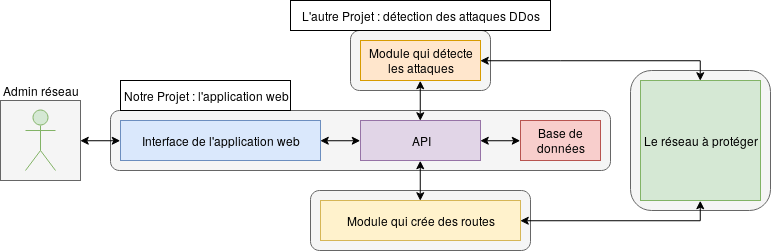
\includegraphics[width=\textwidth]{use_cases.png}
    \caption{Diagramme d'utilisation de l'application}
    \label{fig:use_cases}
\end{figure}

\begin{figure}[H]
    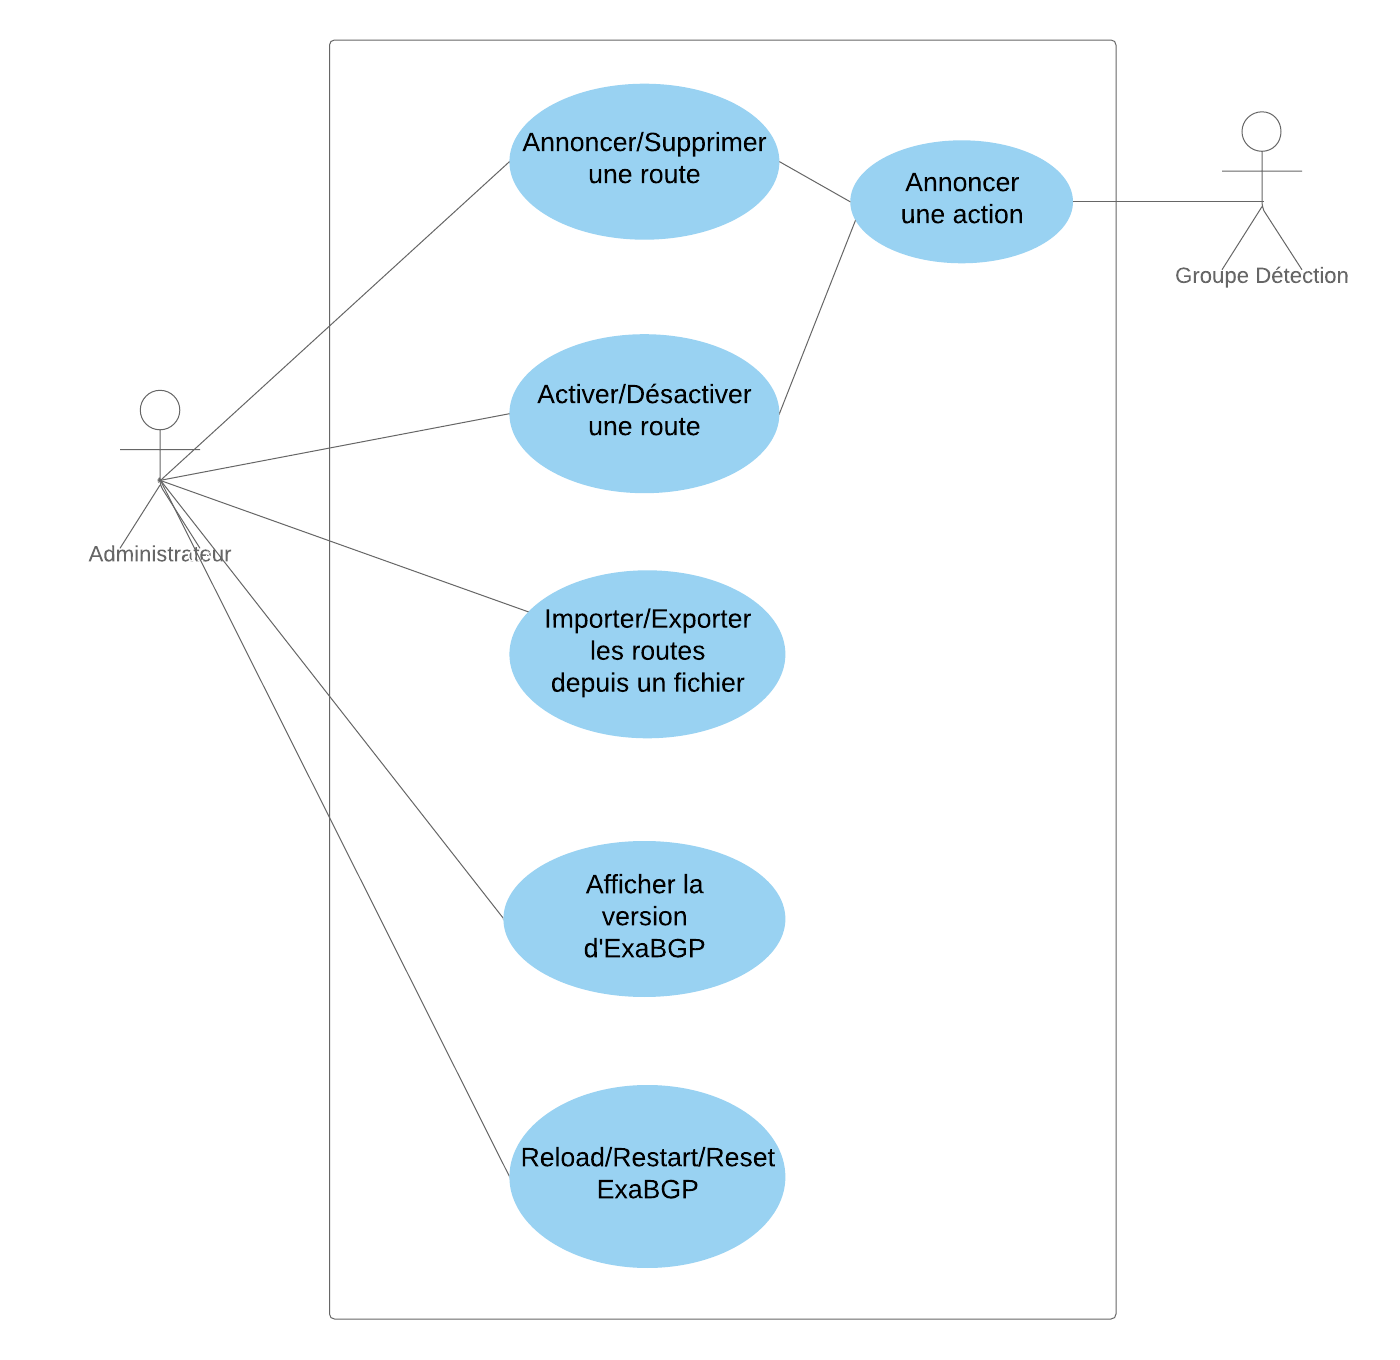
\includegraphics[width=\textwidth]{Blackhole_Use_Cases.png}
    \caption{Diagramme des cas d'utilisation de l'application}
    \label{fig:use_cases_diagramme}
\end{figure}

\newpage

\section{Besoins non fonctionnels}

\subsection{Coût}
Le développement de l'application ne devra entraîner aucun coût financier. C'est pourquoi, nous utiliseront que des logiciels open source sauf l'image CISCO qui nous sera fournie par le client .

\subsection{Performance}
L'application devra être développée pour permettre une défense sur plusieurs attaques simultanées. De plus, l'action décidée par l'administrateur doit pouvoir se faire rapidement. % il faut chiffrer

\subparagraph{Protocole de test :}
\begin{itemize}
    \item Attaque d'au minimum 2 sources.
\end{itemize}
\subparagraph{Résultat obtenu :}
    \begin{itemize}
    \item Routage vers trou noir de tous les trafics attaquants.
\end{itemize}
\subparagraph{Conclusion :}Ce besoin est correctement rempli.

\subsection{Authentifié}
L’application ne devra être utilisable que par l'administrateur. Donc, nous devons donc en place un service d'authentification pour permettre à l'administrateur seulement d'y avoir accès.

\subparagraph{Protocole de test :}
\begin{itemize}
    \item Accès à l'application avec login.
    \item Accès à l'application sans login.
    \item Changement de mot de passe.
\end{itemize}
\subparagraph{Résultat obtenu :}
    \begin{itemize}
    \item Accès sans login rejeté.
    \item L'administrateur peut se connecter.
    \item L'administrateur peut se déconnecter.
    \item L'administrateur peut changer de mot de passe.
\end{itemize}
\subparagraph{Conclusion :}Ce besoin est correctement rempli.

\subsection{Tester}
L'application sera testée sur un réseau virtuel avec au minimum deux routeurs, une machine serveur et une machine cliente et attaquante. Les tests ne s'effectueront que sur le système d'exploitation debian.

\subsection{Fiabilité}
L'application devra être couverte par des tests pour vérifier que les différentes actions sur les routes sont bien implémentées et permettent donc bien de gérer un routage vers trou noir. C'est pourquoi, les tests doivent couvrir le code à hauteur de 80\%.

\subparagraph{Protocole de test :}
\begin{itemize}
    \item Test de couverture.
\end{itemize}
\subparagraph{Résultat obtenu :}
    \begin{itemize}
    \item Code couvert au minimum à 80 \%.
\end{itemize}
\subparagraph{Conclusion :}Ce besoin est correctement rempli.
